\documentclass{article}
\usepackage[utf8]{inputenc}
\usepackage{natbib}
\usepackage{graphicx}
\usepackage{vmargin}
\usepackage{hyperref}
\usepackage{booktabs}
\usepackage{multirow}
\usepackage{siunitx}
\setpapersize{A4}
\setlength{\parskip}{\baselineskip}%
\setlength{\parindent}{0pt}%

\title{Entregable WEKA}
\author{Laura Rodríguez Navas \\ rodrigueznavas@posgrado.uimp.es}
\date{Abril 2020}

\begin{document}

\maketitle

\section*{Preparación de datos}

Consideramos la base de datos Prostate definida sobre 12600 variables predictivas (todas numéricas) y una variable clase binaria \{tumor, normal\}. Está formada por 136 registros y en ella no existen valores desconocidos. Pero está ordenada en función de la variable clase \{Tumor, Normal\}. Como consecuencia, tenemos que aleatorizar la base de datos. Para ello se aplica un filtro a nivel de registro, concretamente de tipo no supervisado llamado Ramdomize. Usamos la semilla que viene por defecto (42).

A continuación, dividimos la base de datos en un conjunto de entrenamiento, con dos tercios de los registros, y un conjunto de test con un tercio de los registros. Para ello se aplica un filtro a nivel de registro y no supervisado llamado RemoveFolds. Como resultado hemos creado un conjunto de entrenamiento con 90 registros.

Observamos que la distribución de la variable clase en el conjunto de entrenamiento no es uniforme.

\begin{center}
	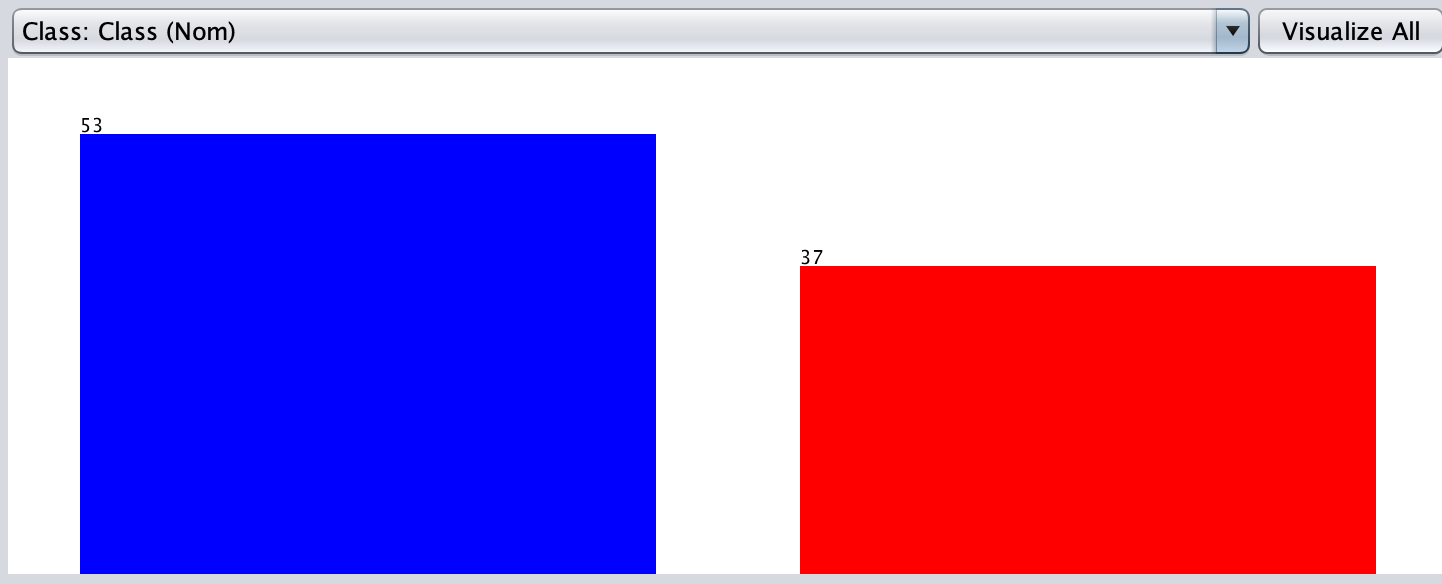
\includegraphics[scale=0.3]{distribucion_norm.png}
\end{center}

\section*{Clasificación}

Se usan los clasificadores Naive Bayes y J48 (C4.5) en una validación cruzada de 5 carpetas (5cv) sobre el conjunto de entrenamiento de la base de datos.

Se han considerado dos parámetros de rendimiento para la evaluación de los resultados. Los parámetros examinados antes y después de la discretización y/o la selección de variables son Accuracy (registros clasificados correctamente) y Error Rate (registros no clasificados correctamente). 

\newpage

\begin{center}
	\begin{tabular}{ |c|c|c| } 
		\hline
		Clasificador & Acc. en \% & ERR en \% \\
		\hline
		Naive Bayes & 52.2222 & 47.7778 \\ 
		J48 (C4.5) & 82.2222 & 17.7778 \\ 
		\hline
	\end{tabular}
\end{center}

Inicialmente y sin la aplicación de alguna mejora, podemos observar que el clasificador J48 (C4.5) clasifica correctamente mucho mejor los registros, en comparación con Naive Bayes. A partir de estos resultados, se puede pensar que se debe a la alta presencia de variables relevantes y redundantes en la base de datos, ya que sabemos que Naive Bayes es un algoritmo sensible en este caso.

\section*{Mejoras}
\subsection*{Discretización}

Primero se prueba un método supervisado a nivel de atributo basado en la entropía. Como resultado, los valores de Accuracy y Error Rate resultantes de la ejecución de los clasificadores después de esta discretización son:

\begin{center}
	\begin{tabular}{cSSSSS}
		\toprule
		\multirow{2}{*}{Clasificador} &
		\multicolumn{2}{c}{Antes Disc.} &
		\multicolumn{2}{c}{Después Disc.} \\
		& {Acc. in \%} & {ERR in \%} & {Acc. in \%} & {ERR in \%} \\
		\midrule
		Naives Bayes & 52.2222 & 47.7778 & 82.2222 & 17.7778 \\
		J48 (C4.5) & 82.2222 & 17.7778 & 87.7778 & 12.2222 \\
		\bottomrule
	\end{tabular}
\end{center}

A continuación, se prueban dos métodos no supervisados a nivel de atributo.

\begin{center}
	\begin{itemize}
		\item Intervalos de igual amplitud. Es el método de discretización no supervisado más simple, que determina los valores mínimo y máximo del atributo discretizado y luego divide el rango en el número definido por el usuario de intervalos discretos de igual amplitud. La tabla siguiente contiene los valores de precisión y tasa de error que dependen del número de bins utilizados (2, 4, 5 y 10). 
		\begin{center}
			\begin{tabular}{cSSSSS}
				\toprule
				\multirow{2}{*}{\# of bins} &
				\multicolumn{2}{c}{Naives Bayes} &
				\multicolumn{2}{c}{J48 (C4.5)} \\
				& {Acc. in \%} & {ERR in \%} & {Acc. in \%} & {ERR in \%} \\
				\midrule
				2 & 51.1111 & 48.8889 & 63.333 & 36.6667 \\
				4 & 54.4444 & 45.5556 & 72.2222 & 27.7778 \\
				5 & 57.7778 & 42.2222 & 68.8889 & 31.1111 \\
				10 & 71.1111 & 28.8889 & 73.3333 & 26.6667 \\
				\bottomrule
			\end{tabular}
		\end{center}
		\item Intervalos de igual frecuencia. Es el método no supervisado que divide los valores ordenados en k intervalos para que cada intervalo contenga aproximadamente el mismo número de instancias de entrenamiento. Por lo tanto, cada intervalo contiene n/k (posiblemente duplicados) valores adyacentes. k es el parámetro predefinido por el usuario. Aquí k representa el número de bins. La tabla siguiente contiene los valores de precisión y tasa de error que dependen del número de bins utilizados (2, 4, 5 y 10). 
		\begin{center}
			\begin{tabular}{cSSSSS}
				\toprule
				\multirow{2}{*}{\# of bins} &
				\multicolumn{2}{c}{Naives Bayes} &
				\multicolumn{2}{c}{J48 (C4.5)} \\
				& {Acc. in \%} & {ERR in \%} & {Acc. in \%} & {ERR in \%} \\
				\midrule
				2 & 65.5556 & 34.4444 & 71.1111 & 28.8889 \\
				4 & 65.5556 & 34.4444 & 80 & 20 \\
				5 & 70 & 30 & 84.4444 & 15.5556 \\
				10 & 72.2222 & 27.7778 & 70 & 30 \\
				\bottomrule
			\end{tabular}
		\end{center}	
	\end{itemize}
\end{center}

Ninguno de los dos métodos no supervisados mejora los resultados del método supervisado, así que se escoge el método supervisado como mejor discretización, debido a la mejor selección de intervalos de forma supervisada y además sin la necesidad de hacer pruebas con distintos intervalos.

El mejor resultado es,

\begin{center}
	\begin{tabular}{cSSSSS}
		\toprule
		\multirow{2}{*}{Clasificador} &
		\multicolumn{2}{c}{Antes Disc.} &
		\multicolumn{2}{c}{Después Disc.} \\
		& {Acc. in \%} & {ERR in \%} & {Acc. in \%} & {ERR in \%} \\
		\midrule
		Naives Bayes & 52.2222 & 47.7778 & 82.2222 & 17.7778 \\
		J48 (C4.5) & 82.2222 & 17.7778 & 87.7778 & 12.2222 \\
		\bottomrule
	\end{tabular}
\end{center}

\subsection*{Selección de variables}

Sabemos que la base de datos contiene muchos atributos, así que primero reduciremos el número de atributos para quedarnos con los 200 mejores y la variable clase, haciendo una selección invariada tipo ranker. Y si además discretizamos con el método supervisado utilizado anteriormente observamos que la clasificación con Naive Bayes mejora muchísimo. Contrariamente, el clasificador J48 (C4.5) empeora. Eso demuestra que al reducir el número de atributos, reducimos el número de variables relevantes y redundantes en la base de datos; que Naive Bayes es un algoritmo sensible en este caso y que J48 (C4.5) no lo es.

La siguiente tabla muestra el análisis anterior,

\begin{center}
	\begin{tabular}{cSSSSS}
		\toprule
		\multirow{2}{*}{Clasificador} &
		\multicolumn{2}{c}{Sin Disc.} &
		\multicolumn{2}{c}{Con Disc.} \\
		& {Acc. in \%} & {ERR in \%} & {Acc. in \%} & {ERR in \%} \\
		\midrule
		Naives Bayes & 52.2222 & 47.7778 & 80 & 20 \\
		J48 (C4.5) & 91.1111 & 8.8889 & 85.5556 & 14.4444 \\
		\bottomrule
	\end{tabular}
\end{center}

Otra mejora que podemos hacer es una selección multivariada de tipo Filter, de método Cfs y voraz con el método de selección hacia delante (forward). En este caso la selección de atributos se ve ampliamente reducida a 18 atributos. También se prueba con discretización y sin discretización.

\begin{center}
	\begin{tabular}{cSSSSS}
		\toprule
		\multirow{2}{*}{Clasificador} &
		\multicolumn{2}{c}{Sin Disc.} &
		\multicolumn{2}{c}{Con Disc.} \\
		& {Acc. in \%} & {ERR in \%} & {Acc. in \%} & {ERR in \%} \\
		\midrule
		Naives Bayes & 58.8889 & 41.1111 & 96.6667 & 3.3333 \\
		J48 (C4.5) & 88.8889 & 11.1111 & 83.3333 & 16.6667 \\
		\bottomrule
	\end{tabular}
\end{center}

\newpage

Finalmente, probamos una selección multivariada de tipo Wrapper para cada clasificador, con el método de selección hacia delante (forward). También se prueba con discretización y sin discretización.

\begin{center}
	\begin{itemize}
		\item Naive Bayes. La selección de atributos se reduce a 2 \{67, 174\}. \\
		\begin{center}
			\begin{tabular}{cSSSSS}
				\toprule
				\multirow{2}{*}{Clasificador} &
				\multicolumn{2}{c}{Sin Disc.} &
				\multicolumn{2}{c}{Con Disc.} \\
				& {Acc. in \%} & {ERR in \%} & {Acc. in \%} & {ERR in \%} \\
				\midrule
				Naives Bayes & 83.3333 & 16.6667 & 82.2222 & 17.7778 \\
				\bottomrule
			\end{tabular}
		\end{center}
		\item J48 (C4.5). La selección de atributos se reduce a 3 \{1, 52, 166\}. \\
		\begin{center}
			\begin{tabular}{cSSSSS}
				\toprule
				\multirow{2}{*}{Clasificador} &
				\multicolumn{2}{c}{Sin Disc.} &
				\multicolumn{2}{c}{Con Disc.} \\
				& {Acc. in \%} & {ERR in \%} & {Acc. in \%} & {ERR in \%} \\
				\midrule
				J48 (C4.5) & 92.2222 & 7.7778 & 86.6667 & 13.3333 \\
				\bottomrule
			\end{tabular}
		\end{center}
	\end{itemize} 
\end{center}

\end{document}
